% \begin{figure}[t]
% \footnotesize
% 	\centering
% \begin{tikzpicture}[x=1.5cm, y=1.5cm, >=stealth]
% \draw (-2.75,4.5) -- (2,4.5);
% %\draw [dotted] (-2.75,5.25) -- (2,5.25);
% \draw (-2.75,4) -- (2,4);
% \draw (-2.75,4.5) -- (-2.75,4);
% \foreach \x/\c in {-2.2/{f}, -1.6/{f-1}, 0.65/{f-n+2}, 1.42/{f-n+1}, 2/{f-n}}
% {
%     \draw (\x,4.5) -- (\x,4);
%     %\node at (\x-0.3, 5.1) {${p_{\c}}$};
%     \node at (\x-0.34, 4.25) {${a_{\c}}$};
% }

% \node (inplogo) at (-0.5,4.75) [,minimum width=5cm,minimum height=0.55cm, align=center] {Input dimension: [$n$ frequency bins,1],\\ $a_f$ - averaged magnitude FFT bin at time t.};,
% \node (inp) at (1.8,4.05) [] {};
% \node (lstm1) at (-0.5,3) [draw,thick,minimum width=7cm,minimum height=0.75cm] {\ac{lstm}-1, 128 cells};
% \node (fc) at (-0.5,2.2) [draw,thick,minimum width=7cm,minimum height=0.75cm] {Fully connected linear layer};
% \node (sm) at (-0.5,1.3) [draw,thick,minimum width=5cm,minimum height=0.75cm] {Softmax layer};
% \node (dummy) at (-0.5,0.4) [draw=none,thick,minimum width=5cm,minimum height=0.75cm] {$\mathbb{P}$(Classes)};
% \foreach \a in {0.1,0.2,0.3,0.9}{
% \draw ($(inp.south)$) edge[out=270,in=90,->] ($(lstm1.north west)!\a!(lstm1.north east)$);
% \draw[->] ($(lstm1.south west)!\a!(lstm1.south east)$) -- ($(fc.north west)!\a!(fc.north east)$);
% \draw ($(fc.south west)!\a!(fc.south east)$) edge[out=270,in=90,->] ($(sm.north west)!\a!(sm.north east)$);
% \draw[->] ($(sm.south west)!\a!(sm.south east)$) -- ($(dummy.north west)!\a!(dummy.north east)$);
% }
% \node at ($(inplogo)!0.8!(lstm1)$) {$\hdots$};
% \node at ($(lstm1)!0.5!(fc)$) {$\hdots$};
% \node at ($(fc)!0.5!(sm)$) {$\hdots$};

% \end{tikzpicture}
% 	\caption{Model-1: Averaged magnitude \ac{fft} \ac{lstm} Model.}

\begin{figure}[htb]
\centering
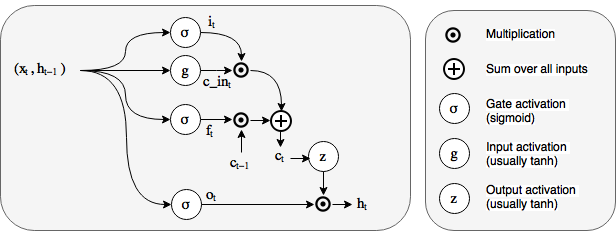
\includegraphics[width=1\columnwidth]{figures/lstm_block.png}
\caption{LSTM cell used in the hidden layers of the model.} 
\label{fig_lstmcell}
\end{figure}

% 	\label{fig_magfft_lstm_model}
% \end{figure}

\begin{figure}[t]
\footnotesize
	\centering
\begin{tikzpicture}[x=1.5cm, y=1.5cm, >=stealth]
\draw (-2.75,5.5) -- (2,5.5);
\draw [dotted] (-2.75,5.25) -- (2,5.25);
\draw (-2.75,5) -- (2,5);
\draw (-2.75,5.5) -- (-2.75,5);

\draw (-2.75,7) -- (2,7);
\draw (-2.75,6.5) -- (2,6.5);
\draw (-2.75,7) -- (-2.75,6.5);

\foreach \x/\c in {-2.2/{f}, -1.6/{f-1}, 0.65/{f-n+2}, 1.42/{f-n+1}, 2/{f-n}}
{
    \draw (\x,7) -- (\x,6.5);
    \node at (\x-0.34, 6.75) {${a_{\c}}$};
}
\node (inplogo0) at (-0.5,7.25) [,minimum width=5cm,minimum height=0.55cm, align=center] {Input dimension: [$n$ frequency bins,1],\\ $a_f$ - averaged magnitude FFT bin at time t.};,

\draw [dashdotted] (-2.75,6.25) -- (2,6.25) node[midway,fill=white] {OR} ;
\foreach \x/\c in {-2.3/{t}, -1.7/{t-1}, 0.7/{t-n+2}, 1.4/{t-n+1}, 2/{t-n}}
{
    \draw (\x,5.5) -- (\x,5);
    \node at (\x-0.3, 5.1) {${p_{\c}}$};
    \node at (\x-0.3, 5.35) {${a_{\c}}$};
}  

\node (inplogo) at (-0.5,5.75) [,minimum width=5cm,minimum height=0.55cm, align=center] {Input dimension: [$n$ timesteps,2],\\ $a_t, p_t$ - amplitude and phase at time t.};
\node (inp) at (1.8,5.05) [] {};
\node (lstm1) at (-0.5,4) [draw,thick,minimum width=7cm,minimum height=0.75cm] {\ac{lstm}-1, 128 cells};
\node (lstm2) at (-0.5,3.1) [draw,thick,minimum width=7cm,minimum height=0.75cm] {\ac{lstm}-2, 128 cells};
\node (fc) at (-0.5,2.2) [draw,thick,minimum width=7cm,minimum height=0.75cm] {Fully connected linear layer};
\node (sm) at (-0.5,1.3) [draw,thick,minimum width=5cm,minimum height=0.75cm] {Softmax layer};
\node (dummy) at (-0.5,0.4) [draw=none,thick,minimum width=5cm,minimum height=0.75cm] {$\mathbb{P}$(Classes)};
\foreach \a in {0.1,0.2,0.3,0.9}{
\draw ($(inp.south)$) edge[out=270,in=90,->] ($(lstm1.north west)!\a!(lstm1.north east)$);
\draw[->] ($(lstm1.south west)!\a!(lstm1.south east)$) -- ($(lstm2.north west)!\a!(lstm2.north east)$);
\draw[->] ($(lstm2.south west)!\a!(lstm2.south east)$) -- ($(fc.north west)!\a!(fc.north east)$);
\draw ($(fc.south west)!\a!(fc.south east)$) edge[out=270,in=90,->] ($(sm.north west)!\a!(sm.north east)$);
\draw[->] ($(sm.south west)!\a!(sm.south east)$) -- ($(dummy.north west)!\a!(dummy.north east)$);
}
\node at ($(inplogo)!0.8!(lstm1)$) {$\hdots$};
\node at ($(lstm1)!0.5!(lstm2)$) {$\hdots$};
\node at ($(lstm2)!0.5!(fc)$) {$\hdots$};
\node at ($(fc)!0.5!(sm)$) {$\hdots$};

\end{tikzpicture}
	\caption{Two layer \ac{lstm} model for classification. The model is trained and deployed for modulation classification using either amplitude-phase signal or the averaged magnitude-FFT signal as input.}
	\label{fig_iq_lstm_model}
\end{figure}

The proposed \ac{lstm} model, that works on the time domain amplitude and phase signal, is introduced in the following subsection. In addition, the baseline \ac{cnn} model used for comparisons is also detailed.
\subsection{LSTM primer}
\label{lstm_primer}
\ac{rnn} are heavily used for learning persistent features from time series data. \ac{lstm} \cite{Hochreiter:lstm} is a special type of \ac{rnn} which is efficient in learning long-term dependencies. The block diagram of a basic version of a \ac{lstm} cell is presented in Figure~\ref{fig_lstmcell} along with the corresponding equations (2-7).


\begin{itemize}
\item Gates
\begin{align}
i_t &= \sigma(W_{xi}x_t + W_{hi}h_{t-1} + b_i)\\
f_t &= \sigma(W_{xf}x_t + W_{hf}h_{t-1} + b_f)\\
o_t &= \sigma(W_{xo}x_t + W_{ho}h_{t-1} + b_o)
\end{align}
\item Input transform
\begin{equation}
c\_in_t = tanh(W_{xc}x_t+W_{hc}h_{t-1}+b_{c\_in})
\end{equation}
\item State update
\begin{align}
c_t &= f_t \cdot c_{t-1}+i_t \cdot c\_in_t\\
h_t &= o_t \cdot tanh(c_t)
\end{align}
\end{itemize}



\ac{lstm} cells have an internal state or memory ($c_t$) along with three gates namely input date ($i_t$), forget gate ($f_t$) and output gate ($f_t$). Based on the previous state and the input data the cells can learn the gate weights for the specified problem. This gating mechanism helps \ac{lstm} cells to store information for longer duration thereby enabling persistent feature learning.
\subsection{Model for complex signals}\label{cmplx_lstm_model}
%\vincent{Section IV.A needs some editing. You mention at the beginning that a 2-layer LSTM network is used, but later on, you use models with 1, 2, and 3 layers. You should start by saying that you consider LSTM network of different layers and not 2.}

A \ac{lstm} network with different layers is used for complex data classification as shown in Figure \ref{fig_iq_lstm_model}. The amplitude and phase of the time domain modulated signal are fed to all cells of the \ac{lstm} model as a two dimensional vector, at each time step for classification. The amplitude vector is L2 normalized and the phase, which is in radians is normalized between -1 and 1. The first two layers are comprised of 128 \ac{lstm} cells each. The final output from the second \ac{lstm} layer, a vector of dimension 128, after all time steps, is fed to the last dense layer of the model. The final layer is a dense softmax layer which maps the classified features to one of the 11 output classes representing the modulation schemes. The two layer model is selected after detailed analysis varying the cell size and layer depths which are detailed in Section~\ref{sec_hyperparams}. 

The intuition to use a \ac{lstm} model for classification is based on the fact that different modulation schemes exhibit different amplitude and phase characteristics and the model can learn these temporal dependencies effectively. Even though fading and other real world effects may slightly hamper the characteristics of the signal, we expect the model to classify signals efficiently by learning good fading resistant representations.
%Since the proposed model can work on variable length sequences, it might also turn useful for classifying signals with varying  sample rates or samples per symbol parameter.
Since the proposed model can work on variable length input time domain samples, we expect the model to learn useful symbol rate independent representations for classification. In addition, the importance of the number of \ac{lstm} cells and layer depth are further investigated by varying these parameters. Model classification accuracies are analyzed with varying layer depth from 1 to 3 and number of cells from 16 to 256. We further analyze these aspects in detail in Section~\ref{results}.

\subsection{Baseline \ac{iq} model}
The two layer CNN 8 tap model presented in \cite{baseline} is used as the baseline model for further comparisons. The baseline model uses 256 and 80 filters in the first two convolutional layers respectively. A publicly available training model is used for generating the baseline performance graph \cite{o2016convolutional}. %In \cite{baseline}, the authors also present complex inception modules combining \ac{cnn} and \ac{lstm} modules. In this paper we show that simple \ac{lstm} models can itself achieve good accuracy, if input data is formatted as amplitude and phase (polar coordinates) instead of \ac{iq} samples (rectangular coordinates).

\subsection{Model training and testing}
Each of the datasets mentioned in Tables~\ref{table_rml_dataset} and \ref{table_modrml_dataset} are split into two, one training set and the other testing set. A seed is used to generate random mutually exclusive array indices, which are then used to split the data into two ascertaining the training and testing sets are entirely different. The number of the training and testing vectors are listed in the corresponding tables. A softmax cross entropy with logits\footnote{https://www.tensorflow.org/api\_docs/python/tf/nn/softmax\_cross\_\\entropy\_with\_logits}, that measures the probability error in discrete classification tasks in which the classes are mutually exclusive, is used as the loss function. Stochastic gradient descent with a minibatch size of 400 vectors is used to avoid local optima. We use the Adam optimizer \cite{adam_optimizer}, a first-order gradient based optimizer with a learning rate of 0.001. The complex two layer \ac{lstm} network is trained for 70 epochs which takes around an hour of training time on a x86 PC with Nvidia GeForce GTX 980 Ti graphics card. We use a basic \ac{lstm} cell with starting training forget bias set to one. While initializing the network, it is helpful to keep the scale of the input variance constant, so that it does not explode or diminish by reaching the final layer. To achieve this \ac{lstm} weights are initialized with a default uniform unit scaling initializer which generates weights with a uniform variance. All the models use the same training parameters unless specified explicitly.

%The proposed complex \ac{lstm} model is also trained using the generated modulation dataset mentioned in Section~\ref{dataset} which contains signals with 4 and 8 samples per symbol. In order to evaluate the robustness of this model, we train the network using dataset with varying SNR from -10dB to +20dB with sample lengths varying from 128 to 512 samples. 

\subsection{Implementation details}\label{implementation}
The neural network is implemented using TensorFlow \cite{tensorflow}, a data flow graph based numerical computation library from Google. Python and C++ bindings of Tensorflow makes the usage of the final trained model easily portable to host based SDR frameworks like GNU Radio \cite{gnuradio_web}. The trained model can be easily imported as a block in GNU Radio which can be readily used in practice with any supported hardware front-end.